\documentclass{article}
\usepackage{amsmath}
\usepackage{tikz}
\usetikzlibrary{matrix}

\begin{document}

\begin{figure}[h]
    \centering
    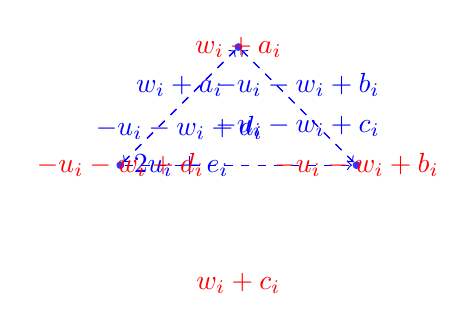
\begin{tikzpicture}[scale=1.5]
        % Define coordinates for the nodes
        \node[circle, fill=blue!80, inner sep=1pt] (A) at (0, 0) {};
        \node[circle, fill=blue!80, inner sep=1pt] (B) at (-1, -1) {};
        \node[circle, fill=blue!80, inner sep=1pt] (C) at (1, -1) {};
        
        % Draw the arrows and labels
        \draw[->, blue, dashed] (A) -- node[above] {$w_i + a_i$} (B);
        \draw[->, blue, dashed] (A) -- node[above] {$-u_i - w_i + b_i$} (C);
        \draw[->, blue, dashed] (B) -- node[below] {$-u_i - w_i + d_i$} (A);
        \draw[->, blue, dashed] (C) -- node[below] {$-u_i - w_i + c_i$} (A);
        \draw[->, blue, dashed] (B) -- node[left] {$2u_i + e_i$} (C);
        
        % Labels for the nodes
        \node[red] at (0, 0) {$w_i + a_i$};
        \node[red] at (-1, -1) {$-u_i - w_i + d_i$};
        \node[red] at (1, -1) {$-u_i - w_i + b_i$};
        \node[red] at (0, -2) {$w_i + c_i$};
    \end{tikzpicture}
    \caption{Graphical rule to parametrize the $Y$-variables in terms of $q$-Weyl algebra generators in the vicinity of the crossing $i$ (center) of the wiring diagram (black). A $Y$-variable situated at a vertex (blue circle) of the symmetric butterfly quiver acquires factors ${\mathrm e}^{a_i+ w_i}$, ${\mathrm e}^{b_i-u_i-w_i}$, ${\mathrm e}^{c_i+w_i}$, ${\mathrm e}^{d_i-u_i-w_i}$ from the neighboring crossing $i$ of the wiring diagram if the vertex is located at the north, east, south, west of $i$, respectively. A $Y$-variable on the vertex $i$ is ${\mathrm e}^{e_i+2u_i}$. The ordering of these factors from different $i$'s (if any) is inconsequential due to the commutativity of the associated canonical variables.}
    \label{fig:quiver_factors}
\end{figure}

\end{document}